\documentclass{article}
\usepackage[utf8]{inputenc}
\usepackage[left=.5in,
			right=.5in,
			bottom=.5in,
			top=.75in]{geometry}
\usepackage{enumitem}
\usepackage{listings}
\usepackage{fancyhdr}
\usepackage{courier}
\usepackage{multicol}
\usepackage{graphicx}
\usepackage{makecell}
\usepackage{multirow}
\usepackage{forest}
\usepackage{amsmath}
\usepackage{amssymb}
\usepackage{tabularx}

\renewcommand{\tt}{\ttfamily \small}
\newcommand{\tabitem}{~~\llap{\textbullet}~~}
\newcolumntype{Y}{>{\centering\arraybackslash}X}

\lstset{
        basicstyle=\ttfamily,
        breaklines=true,
        numbers=left,
        language=python,
        showstringspaces=false,
        keywordstyle=\color{deepblue},
        emphstyle=\color{deepred},    % Custom highlighting style
        stringstyle=\color{deepgreen},
    }

\setlist{noitemsep, topsep=0pt}

\pagestyle{fancy}
\fancyhf{}
\rhead{Page \thepage}   
\lhead{Ben Kettle}
\fancyhead[C]{6.003 Cheat Sheet}

\begin{document}
\section{Math Facts}
\begin{tabularx}{\textwidth}{YYY}
	$\displaystyle \sum_{k=0}^{n-1} ar^k = \left(\frac{1-r^n}{1-r}\right)$ & 
	$\displaystyle \sum_{k=0}^{\infty} ar^k = \frac{a}{1-r}$ &
	$\displaystyle \sum_{i=1}^{n} i = \frac{n(n+1)}{2}$

\end{tabularx}
\section{Properties of Signals}
\begin{multicols}{2}
\subsection{Complex Exponentials}
We can represent signals as complex exponentials to make them a lot easier in certain cases (multiplication). 
\[ e^{jx} = \cos(x) + j\sin(x) \]
\[ cos(x) = \frac{e^{jx} + e^{-jx}}{2} \]
\[ sin(x) = \frac{e^{jx} - e^{-jx}}{2j} = -\frac{j}{2}\left(e^{jx}-e^{-jx}\right) \]
\subsection{Sampling}
Because multiple frequencies can alias to the same frequency when sampled, we use the \textit{Baseband} to describe the frequency represented by a set of samples. The baseband is the range of frequencies $0 \leq \Omega \leq \pi$.

If there are frequencies in the CT signal greater than the Nyquist frequency $f_N = \frac{f_s}{2}$, they will alias to frequencies in the base band. To avoid distortion, remove these frequencies before sampling (anti-aliasing).
\end{multicols}


\section{Fourier Series}

\begin{multicols}{2}
\subsection{Continuous Time Fourier Series}
Split a signal up into harmonically related sinusoids, which each have a frequency that is an integer multiple of the \textit{fundamental frequency} $\omega_0 = \frac{2\pi}{T}$ of the signal. The fundamental frequency has the same period as the \textit{fundamental period} of the signal, or the smallest value $T$ for which $x(t) = x(t+T)$ holds.
\begin{itemize}
	\item Represents periodic signals 
	\item Can't perfectly represent discontinuities---results in Gibb's Phenomenon (overshoot)
		\begin{itemize}
			\item as number of terms increases, width of overshoot gets smaller, but magnitude does not (around 9\%).
		\end{itemize}
\end{itemize}

\[ f(t) = \sum_{k=0}^{\infty} (c_k \cos(k\omega_0 t) + d_k\sin(k\omega_0 t)) \]
\[ c_0 = \frac{1}{T}\int_T f(t) dt \qquad \text{"average"} \]
\[ c_k = \frac{2}{T}\int_T f(t) \cos(k\omega_o t) dt \]
\[d_k = \frac{2}{T}\int_T f(t) \sin(k\omega_o t) dt \]

Using exponential form, we get a simpler set of equations for CTFS:

\[ x(t) = x(t+T) = \sum_{k=-\infty}^{\infty} X[k] e^{j\frac{2\pi k t}{T}} \]
\[ X[k] = \frac{1}{T}\int_T x(t) e^{-j\frac{2\pi kt}{T}}\; dt \]

\subsubsection{Properties}
\begin{itemize}
	\item \textbf{Real-Valued Periodic Signal:} $F[k] = F^*[-k]$ for real-valued signals.
	\item \textbf{Symmetric and Antisymmetric Parts}: The real part of $F[k]$ comes from the symmetric part of the signal, the imaginary part comes from the antisymmetric part of the signal. In trig form, symmetric in $c_k$, antisymmetric in $d_k$.
\end{itemize}
\[ \begin{array}{rcc}
	\textbf{property} & \mathbf{y(t)} & \mathbf{Y[k]} \\
	\hline
	\text{Linearity} & Ax_1(t) + Bx_2(t) & AX_1[k] + BX_2[k] \\
	\text{Time Flip} & x(-t) & X[-k] \\
	\text{Time Shift} & x(t-t_0) & e^{-j\frac{2\pi kt_0}{T}} X[k] \\
	\text{Time Derivative} & \frac{d}{dt} x(t) & Y[k] = j\frac{2\pi}{T} X[k] \\
\end{array} \]

\subsection{DTFS}
In CTFS, there can be an infinite number of harmonics, as resolution is infinite. In a DT signal with period $N$, there can only be $N$ harmonics--the others will alias to a harmonic within those $N$. We have a similar fundamental frequency $\Omega_0 = \frac{2\pi}{N}$.
\[ x[n] = x[n+N] = \sum_{k=k_0}^{k_0 + N -1} X[k] e^{j\frac{2\pi}{N} kn} \]
\[ X[k] = X[k+N] = \frac{1}{N}\sum_{n=n_0}^{n_0+N-1} x[n] e^{-j\frac{2\pi}{N} kn} \]
\subsubsection{Properties}
\[ \begin{array}{rcc}
	\textbf{property} & \mathbf{y[t]} & \mathbf{Y[k]} \\
	\hline
	\text{Linearity} & Ax_1[n] + Bx_2[n] & AX_1[k] + BX_2[k] \\
	\text{Time Flip} & x[-n] & X[-k] \\
	\text{Time Shift} & x[n-m] & e^{-j\frac{2\pi km}{N}} X[k] \\
	\text{Sym. Part} & \frac{1}{2}(x[n] + x[-n]) & Re(X[k]) \\
	\text{Antisym. Part} & \frac{1}{2}(x[n] - x[-n]) & j\cdot Im(X[k])
\end{array} \]

\end{multicols}

\newpage
\begin{multicols}{2}
\section{Fourier Transforms}
\subsection{CT Fourier Transform}
Essentially, a fourier series as the period approaches infinity.
\[ x(t) = \frac{1}{2\pi} \int_{-\infty}^{\infty} X(\omega)\cdot e^{j\omega t} d\omega \quad X(\omega) = \int_{-\infty}^{\infty} x(t) \cdot e^{-j\omega t} dt \]

\subsubsection{Useful Signals}
Stretching in time compresses in frequency, and vice versa.
\begin{center}
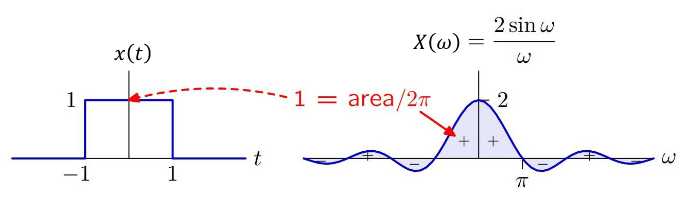
\includegraphics[scale=.6]{ctft_rectangular_pulse.png}
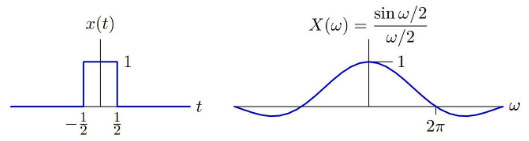
\includegraphics[scale=.75]{ctft_rectangular_pulse_compressed.png}
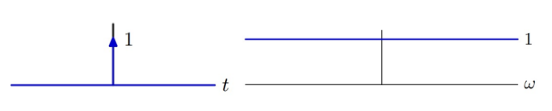
\includegraphics[scale=.75]{ctft_impulse.png}
\end{center}

\subsubsection{Duality}
If taking the CTFT of $x(t)$ gives us $X(\omega)$, then if we interpret those coefficients as another signal and take the CTFT again, we will get $2\pi x(-\omega)$. Need clarity here.

\subsubsection{Properties}
\[
\begin{array}{rcc}
	\textbf{property} & \mathbf{y(t)} & \mathbf{Y(\omega)} \\
	\hline
	\text{Linearity} & ax_1(t) + bx_2(t) & aX_1(\omega) + bX_2(\omega) \\
	\text{Time Reversal} & x(-t) & X(-\omega) \\
	\text{Time Delay} & x(t-t_0) & e^{-j\omega t_0} X(\omega) \\
	\text{Conjugation} & x^*(t) & X^*(-\omega) \\
	\text{Scaling Time} & x(at) & \frac{1}{|a|}X\left(\frac{\omega}{a}\right) \\
	\text{Time Derivative} & \frac{dx(t)}{dt} & j\omega X(\omega) \\
	\text{Freq. Derivative} & tx(t) & j\frac{d}{d\omega} X(\omega)
\end{array}
\]

\subsection{Discrete Time Fourier Transform}
Same idea, we make a periodic version of $x[n]$ by summing shifted copies and take the DTFS of that, but do so as the distance between copies approaches infinity.
\[ x[n] = \frac{1}{2\pi}\int_{2\pi} X(\Omega) \cdot e^{j\Omega n} d\Omega \]
\[ X(\Omega) = X(\Omega + 2\pi) = \sum_{n=-\infty}^{\infty} x[n]\cdot e^{-j\Omega n} \]

\subsubsection{Properties}
Note that the coefficients are periodic in this case
\[
\begin{array}{rcc}
	\textbf{property} & \mathbf{y(t)} & \mathbf{Y(\omega)} \\
	\hline
	\text{Linearity} & ax_1[n] + bx_2[n] & aX_1(\Omega) + bX_2(\Omega) \\
	\text{Time Reversal} & x[-n] & X(-\Omega) \\
	\text{Time Delay} & x[n-n_0] & e^{-j\Omega n_0} X(\Omega) \\
	\text{Conjugation} & x^*[n] & X^*(-\Omega) \\
	\text{Freq. Derivative} & nx[n] & j\frac{d}{d\Omega} X(\Omega)
\end{array}
\]

\section{Discrete Fourier Transform}
Everything so far has had either infinite sums or a continuous domain---difficult for a computer. To solve this, we take an $N$-sample window of the signal, pretend the signal is periodic in $N$, and generate the DTFS of this fake-periodic signal. 
\begin{itemize}
	\item Increasing $N$ increases frequency resolution
	\item If the signal is not periodic in $N$, we get spectral blurring where frequencies do not line up exactly with the positions of the coefficients. 
\end{itemize}

\[ x[n] = \sum_{k=0}^{N-1} X[k] e^{j\frac{2\pi k}{N} n} \qquad X[k] = \frac{1}{N} \sum_{n=0}^{N-1} x[n]\cdot e^{-j\frac{2\pi k}{N} n} \]

\subsubsection{Properties}
\[ \begin{array}{rcc}
	\textbf{property} & \mathbf{y(t)} & \mathbf{Y[k]} \\
	\hline
	\text{Linearity} & Ax_1[n] + Bx_2[n] & AX_1[k] + BX_2[k] \\
	\text{Time Flip} & x_p[N-n] & X[-k] \\
	\text{Time Shift} & x[n-n_0] & e^{-j\frac{2\pi k}{N}n_0} X[k] \\
	\text{Freq. Shift} & e^{-j\frac{2\pi k_0}{N}n}\cdot x[n] & X[k-k_0] \\
	\text{Conjugation} & x^*[n] & X^*[-k] \\
\end{array} \]

\section{Systems Abstraction}
Many applications can be modeled as systems that convert an input signal to an output signal. We focus on systems that are \textbf{linear} (you can add them together) and \textbf{time invariant} (delaying input delays the output by the same amount). 

Systems can be represented with a \textbf{difference equation} ($y[n] = \frac{x[n] + x[n-1]}{2}$ or in terms of \textbf{convolution} (using its unit-sample response). With convolution, we can use linearity to then construct the output of any signal by just adding and shifting.

\subsection{Convolution}
Given a unit-sample response for a system, we can compute the output signal by shifting, multiplying, and adding, or integrating for a CT system:
\[ y[n] = (x * h)[n] = \sum_{k=-\infty}^{\infty} x[k]h[n-k] \]
\[ y(t) = (x*h)(t) = \int_{-\infty}^{\infty}x(\tau)h(t-\tau)\; d\tau \]
Convolution is \textbf{commutative} (can change the order), \textbf{associative} (which pair you convolve first doesn't matter) and \textbf{distributive over addition}.
\end{multicols}
\end{document}
